%
% Errors in Quantum Networks
%

\section{Errors in quantum networks} \label{sec:errors_in_nets} \index{Errors in quantum networks}

\dropcap{A}{s} with classical data, quantum data is susceptible to corruption during transmission. However, in addition to all the usual classical error models, quantum information is subject to further uniquely quantum errors. These errors can be represented using the quantum process formalism and fully characterised using QPT (Sec.~\ref{sec:QPT}). We now briefly discuss several of the dominant errors arising in quantum systems, paying especial attention to error models acting on qubits and optical states, as these are the most relevant in a quantum networking context.

%
% Known Unitaries
%

\subsection{Known unitaries} \index{Unitary!Errors}

The most trivial error mechanism is when a (potentially multi-qubit) unitary channel (e.g an identity channel for the purposes of quantum memory) actually implements some unitary transformation, $\hat{U}$, that is not that which is desired. However, the unitary is constant, not varying from trial to trial, and is known, which can be easily determined by performing QPT on the channel. For example, an optical fibre might induce a polarisation rotation on transmitted photons, but the fibre isn't changing and neither is the rotation. If consistently implementing the same known unitary then reversing it is straightforward in most architectures, by applying $\hat{U}^\dag$, since $\hat{U}^\dag\hat{U}=\hat{\mathbb{I}}$.

%
% Unknown Unitaries
%

\subsection{Unknown imperfect unitaries} \index{Unitary!Errors}

Alternate to known unitaries, the unitary operation implemented by a node/channel may deviate from that which is desired, in an unknown manner, thereby implementing a slightly different operation than that which we intended to engineer. Specifically, the effective unitary can be represented as the ideal unitary, augmented by some deviation matrix,
\begin{align}
	\hat{U}_\mathrm{effective} = \hat{U}_\mathrm{ideal} + \hat{\Delta}_\mathrm{error},
\end{align}
where the matrix elements of $\hat{\Delta}_\mathrm{error}$ (which is not unitary in general) are unknown, but hopefully small. Since the unknown deviation matrix needn't be constant, it will be a function of random variables, evaluated independently for each trial of the process. Furthermore, since the deviation matrix may vary from trial to trial, QPT cannot be employed to characterise it, unlike unitaries with fixed errors.

%
% Loss
%

\subsection{Loss} \label{sec:eff_err} \index{Loss!Channel}

Given that quantum communication links will typically be optical, the dominant error mechanism is likely to be loss. We let the \textit{efficiency}, $\eta$, of an optical quantum process be the probability that a given photon entering the channel leaves the channel in the desired mode, or probability \mbox{$1-\eta$} of being lost. In the case of information encoded into single-photon states, e.g using the polarisation degree of freedom, $\eta$ corresponds exactly to the success probability of the communication.

When implementing protocols employing post-selection upon detecting all photons, the protocol will be non-deterministic, where loss dictates the protocol's success probability. Specifically, with $n$ photons, each with efficiency $\eta$, the net post-selection success probability\index{Post-selection success probability} of the entire device is,
\begin{align}
	P=\eta^n.
\end{align}
This implies an exponential number of trials\index{Trials},
\begin{align}
	N=\left(\frac{1}{\eta}\right)^n,
\end{align}
is required in post-selected protocols. Clearly this exponential scaling is of concern, requiring demanding efficiencies in future large-scale implementations.

% Model

\subsubsection{Model}\index{Loss model}

Formally, let $\mathcal{E}^\mathrm{loss}_\eta$ be the loss channel with efficiency $\eta$. The channel acting on an initially pure single-photon state, $\ket{1}$, can be modelled as a beamsplitter with transmissivity $\eta$ acting on the state, where the reflected mode is traced out, shown in Fig.\ref{fig:loss_model}. This yields the quantum process,
\begin{align}
\mathcal{E}^\mathrm{loss}_\eta(\hat\rho) = \mathrm{tr}_B[\hat{U}_\mathrm{BS}(\hat\rho_A\otimes\ket{0}_B\bra{0}_B)\hat{U}_\mathrm{BS}^\dag],
\end{align}
where $\hat{U}_\mathrm{BS}$ is the beamsplitter operation.

\begin{figure}[!htbp]
	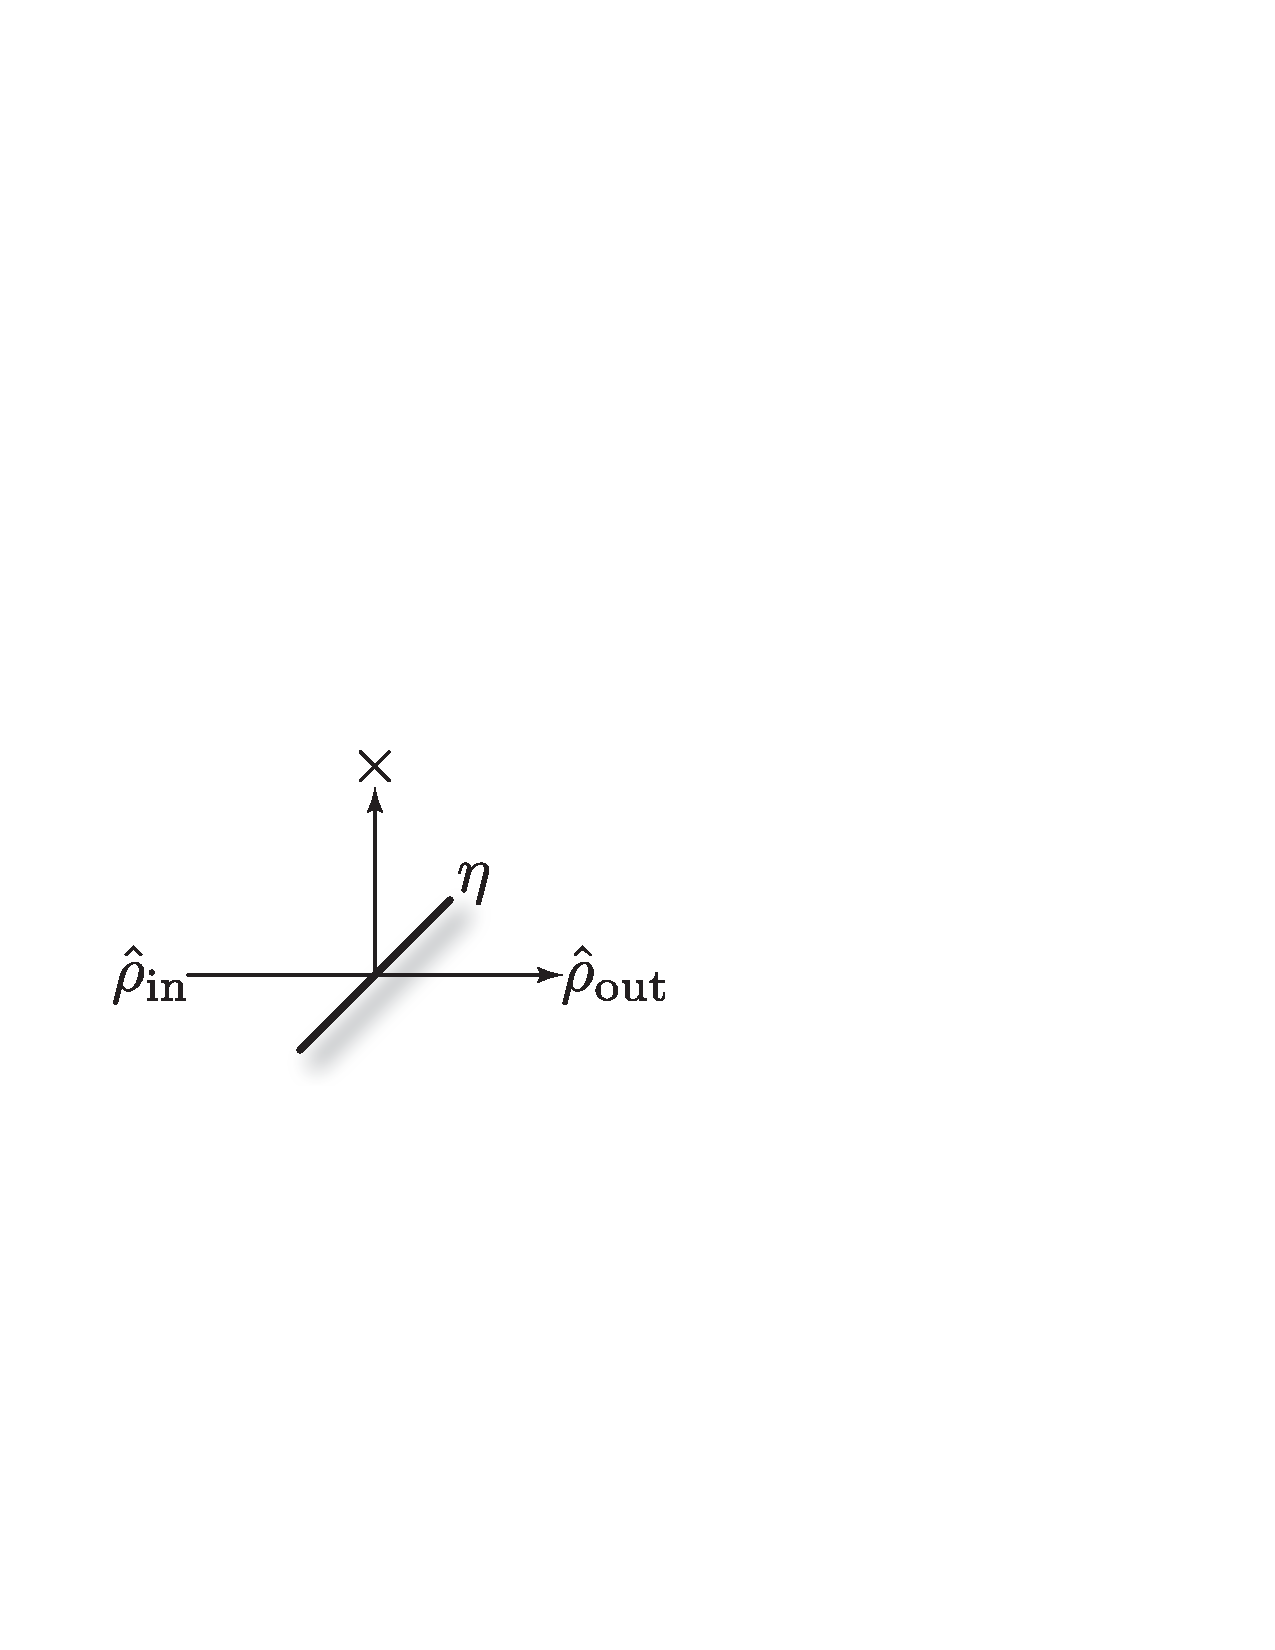
\includegraphics[clip=true, width=0.3\textwidth]{loss_model}
	\captionspacefig \caption{Model for the loss channel. The input state, $\hat\rho$, passes through a beamsplitter of transmissivity $\eta$, and the reflected mode discarded, yielding the lossy output state \mbox{$\mathcal{E}^\mathrm{loss}_\eta(\hat\rho)$}.} \label{fig:loss_model} \index{Loss!Channel}
\end{figure}

Consecutive loss channels act multiplicatively,
\begin{align}
\mathcal{E}_{\eta_1}^\mathrm{loss} \circ \mathcal{E}_{\eta_2}^\mathrm{loss} = \mathcal{E}_{\eta_1 \eta_2}^\mathrm{loss}.
\end{align}

% Linear optics networks

\subsubsection{Linear optics networks}\index{Linear optics networks}

In the special case of linear optics circuits, loss channels have the elegant property that, provided the loss rate is uniform across all modes, they can be commuted through the circuit to the front or back \cite{???}\index{Loss!Commutation}. Specifically,
\begin{align}
(\mathcal{E}_{\eta}^\mathrm{loss})^{\otimes m} \circ \mathcal{E}_U = \mathcal{E}_U \circ (\mathcal{E}_{\eta}^\mathrm{loss})^{\otimes m},
\end{align}
where $\mathcal{E}_U$ is a unitary linear optics process, implementing a photon-number-preserving map of the form of Eq.~(\ref{eq:LO_unitary_map}). This simplifies the treatment of distinct system inefficiencies (such as source, network and detector inefficiencies) by allowing us to commute them to the beginning or end of the circuit and combine them together into a single net efficiency. In many scenarios, this allows the different system inefficiencies to be dealt with via post-selection.

% Single-photon encoding

\subsubsection{Single-photon encoding}\index{Single-photon encoding}

In the case of the vacuum and single-photon states, which is most common to qubit encodings, we obtain,
\begin{align}
	\mathcal{E}^\mathrm{loss}_\eta(\ket{0}\bra{0}) &= \ket{0}\bra{0}, \nonumber \\
\mathcal{E}^\mathrm{loss}_\eta(\ket{1}\bra{1}) &= (1-\eta)\ket{0}\bra{0} + \eta\ket{1}\bra{1}.
\end{align}
This dynamic is of the same form as amplitude damping (Sec.~\ref{sec:amp_damp}).

% Polarisation & dual-rail encoding

\subsubsection{Polarisation \& dual-rail encoding}\index{Polarisation encoding}\index{Dual-rail encoding}

This process would apply equivalently to both horizontal and vertical polarisations. Therefore, via linearity, the loss channel acting on a polarisation-encoded qubit (Sec.~\ref{sec:single_phot_enc}) yields,
\begin{align}
\mathcal{E}^\mathrm{loss}_\eta(\ket\psi_\mathrm{pol}\bra\psi_\mathrm{pol}) = (1-\eta) \ket{0}\bra{0} + \eta\ket\psi_\mathrm{pol}\bra\psi_\mathrm{pol}.
\end{align}

The same applies in the context of dual-rail encoding. Note that while this transformation mixes the state in the photon-number degree of freedom, it preserves coherence between the horizontal and vertical single-photon components. Thus, upon successful post-selection, the state is projected back onto the desired qubit state.

% Photon-number encoding

\subsubsection{Photon-number encoding}\index{Photon-number encoding}

In the general case of an $n$-photon Fock state, we obtain,
\begin{align}
	\mathcal{E}^\mathrm{loss}_\eta(\ket{n}\bra{n}) = \sum_{i=0}^n \binom{n}{i} \eta^i(1-\eta)^{n-i} \ket{i}\bra{i}.
\end{align}

In the case of higher order photon-number encoding of qudits\index{Qudits}, as per Eq.~(\ref{eq:number_qudit}), the probability of an $n$-photon basis state being maintained scales as $\eta^n$. That is, if the highest photon-number term in our qudit is $n$, that component has an exponentially low probability of being preserved through the loss channel. For this fundamental reason, photon-number encoding does not enable infinite-dimensional qudits to be encoded.

% Coherent state encoding

\subsubsection{Coherent state encoding}\index{Coherent state encoding}

Coherent states are the one example of states, which are in a sense robust against loss, since a lossy coherent state is another coherent state with lower amplitude, but without any loss in coherence,
\begin{align}
\mathcal{E}^\mathrm{loss}_\eta(\ket\alpha\bra\alpha) = \ket{\eta\alpha}\bra{\eta\alpha}.
\end{align}
This arises because coherent states are eigenstates of the photonic annihilation operator, \mbox{$\hat{a}\ket{\alpha}=\alpha\ket{\alpha}$}.

However, although coherence is maintained under the loss channel, the process is irreversible, since noise-free amplitude amplification is not possible in general \cite{???}. Thermal states exhibit the same property, that a loss channel simply yields another thermal state with reduced amplitude, although these exhibit no coherence.

% Cat state encoding

\subsubsection{Cat state encoding}

To the contrary, while cat states (Sec.~\ref{sec:cat_enc}) are simple superpositions of coherent states, they are extremely sensitive to loss. This is because cat states have well-defined photon-number parity (strictly even or odd photon-number), and therefore the loss of just a single photon will flip a cat state to an orthogonal one. Since the probability of photon loss occurring increases exponentially with photon-number, large amplitude cat states are exponentially sensitive to loss channels.

%Consider an even-parity cat state, as per Eq.~(\ref{eq:cat_state_enc}). Subjecting this to a loss channel yields the mixed state,
%\begin{align}
%&\hat\rho_\mathrm{loss} = \mathcal{E}_\eta^\mathrm{loss}(\ket{\mathrm{cat}_+(\alpha)}\bra{\mathrm{cat}_+(\alpha)}) = {\mathcal{N}_+}^2 \nonumber\\
%&\cdot (\ket{\eta\alpha}\bra{\eta\alpha} + \ket{\eta\alpha}\bra{-\eta\alpha} + \ket{-\eta\alpha}\bra{\eta\alpha}+\ket{-\eta\alpha}\bra{-\eta\alpha}),
%\end{align}
%which has purity,
%\begin{align}
%	\mathcal{P} &= \mathrm{tr}({\hat\rho_\mathrm{loss}}^2)\nonumber\\
%	&=
%\end{align}

%\comment{To do}

% NOON states

\subsubsection{NOON states}\index{NOON states}

Similarly, NOON states (Sec.~\ref{sec:NOON}) undergo complete wave-function collapse if just a single photon is lost to the environment, and because there are $N$ photons in total, the probability of wave-function collapse grows exponentially with photon-number.

% Scaling

\subsubsection{Scaling}

The scaling of loss over distance $d$ varies depending on the medium through which the light traverses. We will consider two dominant mediums, most relevant to future quantum networking:
\begin{itemize}
	\item Optical fibre\index{Optical fibres}: mode geometry is well-preserved, but optical medium is intrinsically lossy.
	\item Free-space\index{Free-space}: mode geometry is subject to dispersion\index{Dispersion}, but the medium is either lossless (in vacuum), or very low-loss (in atmosphere).
\end{itemize}

When propagating through fibre (or atmosphere, or some other lossy medium) net efficiency scales inverse exponentially as,
\begin{align}
	\eta = O(e^{-\alpha d}),
\end{align}
where $\alpha$ is a characteristic of the medium\footnote{With present-day fibre technology, this characteristic decay rate is on the order of \mbox{$\alpha = \frac{1}{22\mathrm{km}}$}.}.

In free-space on the other hand, where the medium of propagation is vacuum, which is effectively lossless, the effective loss rate is not determined by the medium, but rather by the fact that the spot-size\index{Spot-size} of an optical state is subject to dispersion\index{Dispersion} and grows only quadratically with distance, as shown in Fig.~\ref{fig:free_space_disp}. Then when the light is detected, if the spot-size is greater than the detector aperture, the undetected component effectively translates to loss. Thus through free-space the effective efficiency scales as,
\begin{align}
	\eta = O\left(\frac{1}{d^2}\right),
\end{align}
which is far more favourable than the exponential scaling inherent to lossy mediums. This provides space-based quantum networks with an inherent competitive advantage compared to any form of ground-based network.

Through atmospheric channels we will have both dispersion and distance-dependent loss, yielding an effective loss rate given by the product of the two effects,
\begin{align}
	\eta = O\left(\frac{e^{-\alpha d}}{d^2}\right).
\end{align}

\begin{figure}[!htbp]
	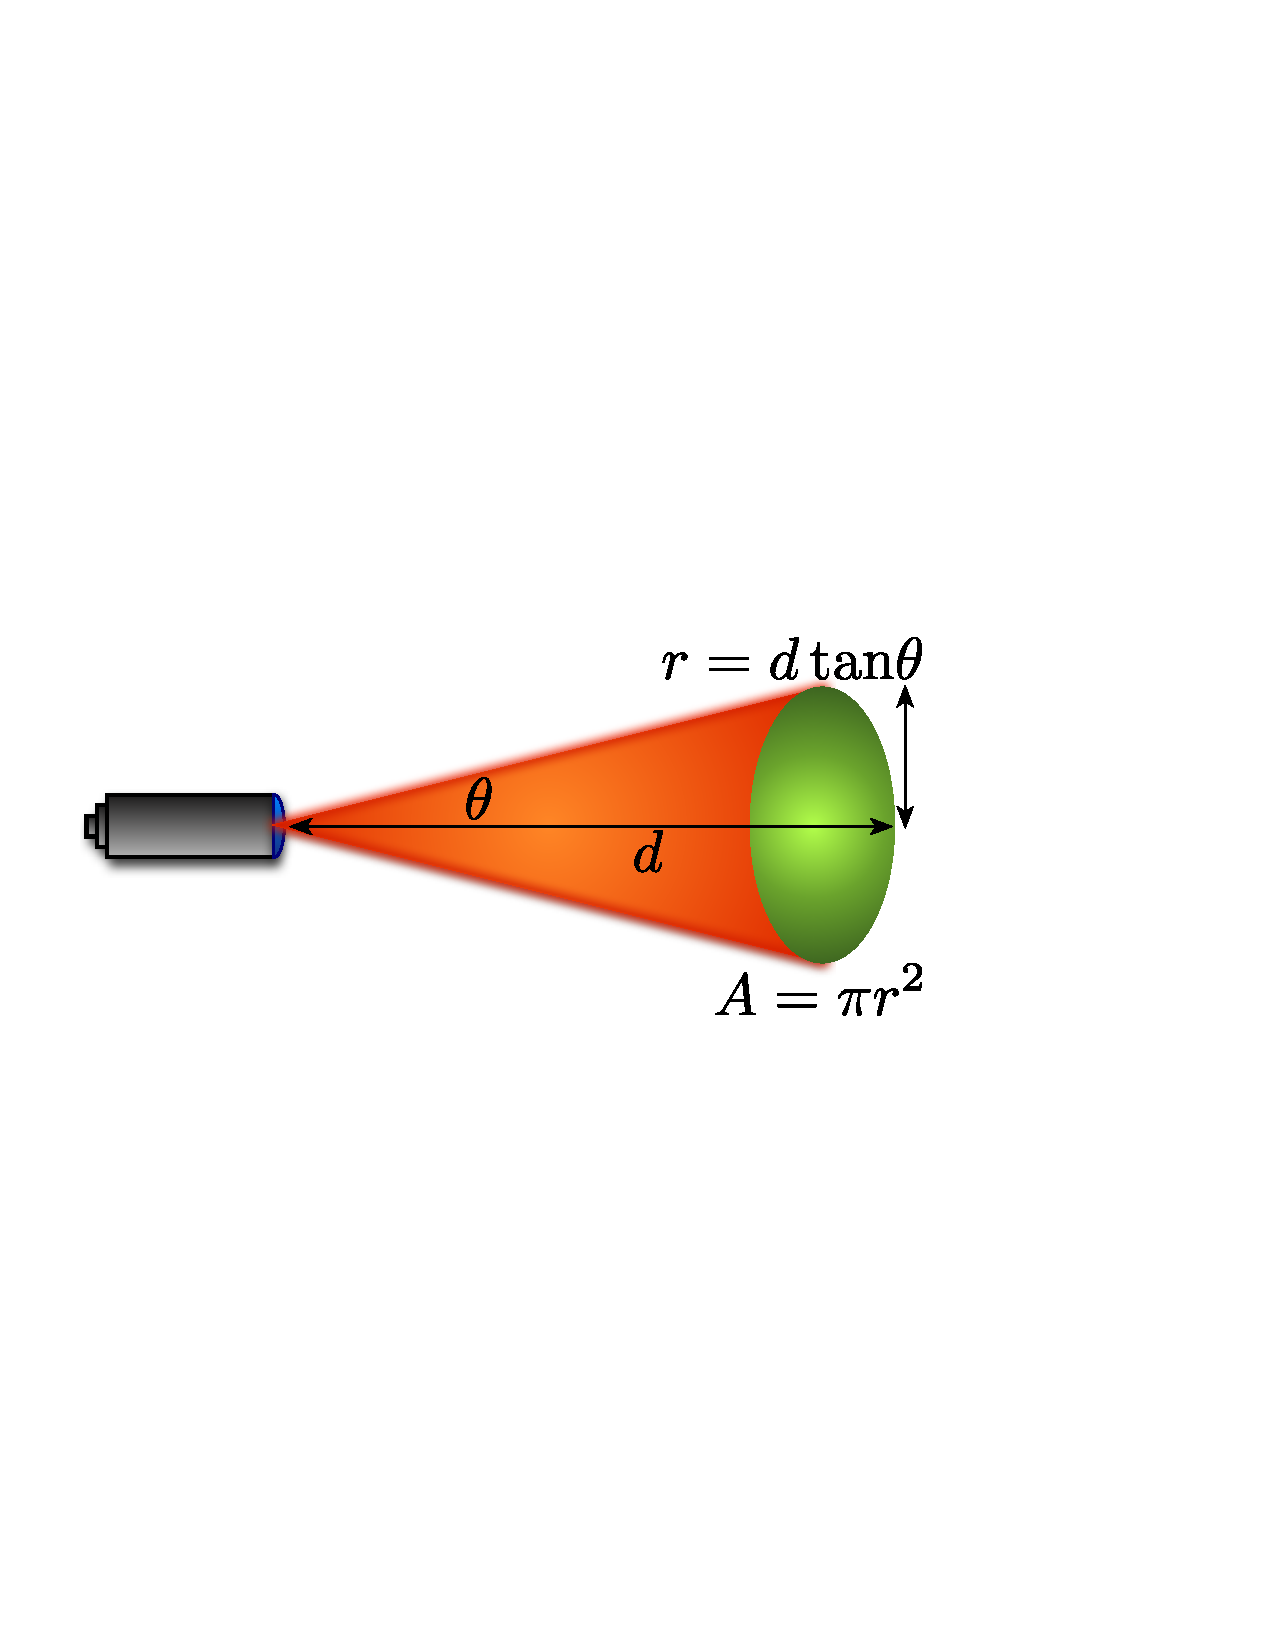
\includegraphics[clip=true, width=0.475\textwidth]{free_space_dispersion}
	\captionspacefig \caption{Spot-size of an optical beam grows quadratically with distance from the source. If the beam is then collected via a camera with aperture area $A'$, any component of $A$ falling outside of $A'$ is effectively lost, yielding an effective loss channel with efficiency \mbox{$\eta = \frac{A'}{A} = \frac{A'}{\pi d^2 \tan^2\theta} = O\left(\frac{1}{d^2}\right)$}.} \label{fig:free_space_disp}
\end{figure}

%
% Dephasing
%

\subsection{Dephasing} \label{sec:dephasing_error} \index{Dephasing!Channel}

The dephasing error model describes the deterioration of quantum coherence in a state. It does not change the actual amplitudes of the components in the superposition, but rather reduces the state to a mixture of those components. Thus, dephasing can be thought of as destroying quantum information (coherence), while retaining classical information (probability amplitudes). 

% Qubits

\subsubsection{Qubits}

In terms of qubits, dephasing is most commonly represented using the Kraus representation\index{Kraus representation},
\begin{align} \label{eq:dephasing_channel}
\mathcal{E}_p^\mathrm{dephasing}(\hat\rho) = p\cdot\hat\rho + (1-p)\cdot \hat{Z}\hat\rho\hat{Z},
\end{align}
where $\hat\rho$ is the state of a single qubit, and $\hat{Z}$ is the Pauli phase-flip operator\footnote{Bit-flip\index{Bit-flip!Channel} and bit-phase-flip\index{Bit-phase-flip channel} channels may be represented similarly by replacing $\hat{Z}$ with $\hat{X}$ or $\hat{Y}$ respectively, although these don't arise as naturally as dephasing in many physical contexts.}. Intuitively this tells us that the dephasing channel creates a mixture of an input state with its phase-flipped self.

An alternate interpretation for the dephasing channel is that it is equivalent to the outside environment measuring $\hat\rho$ in the logical ($\hat{Z}$) basis, but unknown to us, thereby projecting the state onto one basis state or another, yielding a mixture of the two.

Dephasing acting on $\hat\rho$ can be very elegantly visualised as simply nullifying the off-diagonal matrix elements, i.e eliminating coherence terms. Dephasing is a ubiquitous error mechanism and affects all current quantum computing architectures.

Consecutive dephasing channels accumulate into another dephasing channel,
\begin{align} \label{eq:multi_deph}
\mathcal{E}_{p_1}^\mathrm{dephasing} \circ \mathcal{E}_{p_2}^\mathrm{dephasing} = \mathcal{E}_{p'}^\mathrm{dephasing},
\end{align}
where,
\begin{align}
	p' = p_1 p_2 + (1-p_1)(1-p_2),
\end{align}
i.e the probability that an even number of phase-flips have occurred.

As a simple example, consider the \mbox{$p=1/2$} dephasing channel acting on the \mbox{$\ket{+} = \frac{1}{\sqrt{2}}(\ket{0}+\ket{1})$} state. Then we have,
\begin{align}
\mathcal{E}^\mathrm{dephasing}_{1/2}(\ket{+}\bra{+}) &= \frac{1}{2} (\ket{+}\bra{+} + \hat{Z}\ket{+}\bra{+}\hat{Z}) \nonumber \\
&= \frac{1}{2} (\ket{+}\bra{+} + \ket{-}\bra{-}) \nonumber \\
&= \frac{1}{2} (\ket{0}\bra{0} + \ket{1}\bra{1}) \nonumber \\
&= \frac{\mathbb{\hat{I}}}{2},
\end{align}
is the completely mixed state. That is, the state has completely decohered. Note, however, that this complete decoherence depended on the choice of input state. A computational basis state, on the other hand, would be left unchanged by this channel,
\begin{align}
\mathcal{E}^\mathrm{dephasing}_{1/2}(\ket{0}\bra{0}) &= \frac{1}{2} (\ket{0}\bra{0} + \hat{Z}\ket{0}\bra{0}\hat{Z}) \nonumber \\
&= \ket{0}\bra{0}, \nonumber \\
\mathcal{E}^\mathrm{dephasing}_{1/2}(\ket{1}\bra{1}) &= \frac{1}{2} (\ket{1}\bra{1} + \hat{Z}\ket{1}\bra{1}\hat{Z}) \nonumber \\
&= \ket{1}\bra{1}.
\end{align}

Note that the probability of no dephasing occurring over multiple dephasing channels in series is given by the product of the respective probabilities for the individual channels.

% T_2-times

\subsubsection{$T_2$-times}\index{T$_2$-time}

A qubit dephasing channel is often quoted in terms of its $T_2$-time, a characteristic time for dephasing to occur under continuous time-evolution. Specifically, the probability of no dephasing occurring scales as,
\begin{align}
p_\mathrm{no\,error} = e^{-t/T_2},	
\end{align}
yielding a the equivalent dephasing channel,
\begin{align}
\mathcal{E}_t^\mathrm{dephasing}(\hat\rho) = e^{-t/T_2} \hat\rho + \frac{1}{2}(1-e^{-t/T_2})(\hat\rho + \hat{Z}\hat\rho\hat{Z}),
\end{align}
as shown in Fig.~\ref{fig:T2_time}. For a qubit density matrix,
\begin{align}
	\hat\rho = \left(\begin{matrix}{}
 \alpha & \gamma \\
 \gamma^* & \beta
\end{matrix}\right),
\end{align}
this is equivalent to adding a factor of $e^{-t/T_2}$ to the two off-diagonal (coherence) elements,
\begin{align}
	\hat\rho_t = \left(\begin{matrix}{}
 \alpha & e^{-t/T_2}\gamma \\
 e^{-t/T_2}\gamma^* & \beta
\end{matrix}\right).
\end{align}

\begin{figure}[!htbp]
	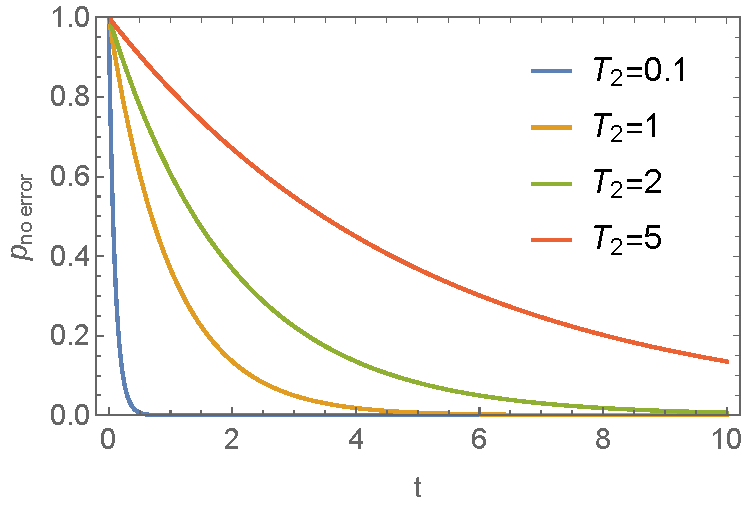
\includegraphics[clip=true, width=0.475\textwidth]{T2_time}
	\captionspacefig \caption{Dephasing under continuous-time evolution, with characteristic decay rate given by the $T_2$-time. $p_\mathrm{no\,error}$ is the probability that the state is left unchanged, whereas \mbox{$1-p_\mathrm{no\,error}$} is the probability that it is replaced with the completely dephased state.}\label{fig:T2_time}
\end{figure}

% Optical states

\subsubsection{Optical states}

The notion of dephasing can be easily generalised to non-qubit states of light, i.e with photon-number \mbox{$n>1$}. In general, dephasing has the property of mapping a superposition of basis states to a mixture of the same basis states, whilst preserving amplitudes. Thus, for perfect dephasing,
\begin{align}
\mathcal{E}^\mathrm{dephasing}\left(\sum_i \alpha_i\ket{i} \cdot \sum_j \alpha_j^*\bra{j} \right) \to \sum_i |\alpha_i|^2 \ket{i}\bra{i},
\end{align}
for some arbitrary basis enumerated by $i$ and $j$. As an example, this process decoheres coherent states into thermal states. For partial dephasing, we can express the channel as creating a mixture over the input state with different phase rotations applied,
\begin{align} \label{eq:deph_int}
\mathcal{E}_{\phi}^\mathrm{dephasing}(\hat\rho) = \int_{0}^{2\pi} \phi(\omega) \hat{\Phi}(\omega)\hat\rho\,\hat{\Phi}(\omega)^\dag\,d\omega,
\end{align}
where $\hat{\Phi}(\omega)$ is a phase-shift operator with phase $\omega$, obeying \mbox{$\hat\Phi(\omega)^\dag = \hat\Phi(-\omega)$}, and $\phi(\omega)$ is a normalised probability density function characterising the distribution of phase-shifts. In the case of optical states, the phase-shift operators take the form,
\begin{align}\index{Phase!Shifts}
\hat\Phi(\omega) = e^{-i\omega\hat{n}},
\end{align}
in the photon-number basis, where $\hat{n}=\hat{a}^\dag\hat{a}$ is the photon-number operator\index{Photon-number operator}, satisfying \mbox{$\hat{n}\ket{n}=n\ket{n}$}. With no dephasing, \mbox{$\phi(\omega)=\delta(\omega)$} and $\mathcal{E}$ reduces to the identity channel. Otherwise, the off-diagonal (coherence) terms in the density operator begin to cancel out, leaving the diagonal (amplitude) terms unchanged. Thus, a perfect dephasing channel acting on a coherent state yields a thermal state of equal amplitude.

From this definition it can be seen that susceptibility to dephasing increases with photon-number, since the number operator adds a multiplicative factor to the acquired phase-shift,
\begin{align}
\hat\Phi(\omega) \ket{n} = e^{-i\omega n}\ket{n}.
\end{align}
For number states not in superposition, this corresponds to a simple unimportant global phase, since number states are phase-invariant. However, in superposition this adds relative phases, thereby destroying coherences upon applying the integral from Eq.~(\ref{eq:deph_int}).

%
% Depolarisation
%

\subsection{Depolarisation} \index{Depolarising channel}

Depolarisation is a noise model more general than dephasing, that probabilistically replaces a state with the completely mixed state (regardless of the input state). That is, with some probability we lose \textit{all} quantum \textit{and} classical information, i.e both coherences and probability amplitudes. Note that the dephasing channel introduced above only destroys quantum coherence, whilst preserving amplitudes. Formally, the depolarising channel can be expressed as,
\begin{align} \label{eq:depolarizing_channel}
\mathcal{E}^\mathrm{depolarising}_p(\hat\rho) = p \cdot \hat\rho + (1-p)\cdot \frac{\mathbb{\hat{I}}}{\mathrm{dim}(\hat\rho)},
\end{align}
where $\mathbb{\hat{I}}/\mathrm{dim}(\hat\rho)$ is the completely mixed state in the $d$-dimensional Hilbert space.

When acting on qubits, the depolarising channel can equivalently be represented as the action of each of the four Pauli matrices with equal probability, since,
\begin{align}
\frac{\mathbb{\hat{I}}}{2} = \frac{1}{4}(\hat\rho + \hat{X}\hat\rho\hat{X} + \hat{Y}\hat\rho\,\hat{Y} + \hat{Z}\hat\rho\hat{Z}).
\end{align}
Thus, both dephasing and depolarisation are examples of Pauli error models.

In the qubit basis (i.e not including loss, for example), the Pauli matrices form a complete basis for quantum operations. Thus, the depolarising channel is the most general qubit error model, since it effectively applies all four Pauli error channels. For this reason, when evaluating fault-tolerance thresholds for QEC codes, thresholds are typically quoted in terms of the depolarising error rate.

Like the dephasing and loss channels, the error probability of multiple channels in series accumulates multiplicatively,
\begin{align}
\mathcal{E}_{p_1}^\mathrm{depolarising} \circ \mathcal{E}_{p_2}^\mathrm{depolarising} = \mathcal{E}_{p_1 p_2}^\mathrm{depolarising}.
\end{align}

%
% Amplitude Damping
%

\subsection{Amplitude damping} \index{Amplitude damping!Channel} \label{sec:amp_damp}

An error not so much relevant to optics, but which arises very naturally in some other systems, such as atomic systems or quantum dots, is amplitude damping, also referred to as a \textit{relaxation channel}. Here the process models the relaxation of a higher energy level, $\ket{1}$, to a lower energy one, $\ket{0}$. The $\ket{0}$ state is assumed to be the ground state and cannot relax any further, but the $\ket{1}$ state can spontaneously relax to the ground state. After complete amplitude damping, any input state will be left in the ground state $\ket{0}$. This model can be thought of as energy dissipating from the qubit system and being measured by the environment, leading to a type of decoherence whereby the input state is probabilistically replaced by the ground state.

The amplitude damping channel is easily represented in the quantum process formalism using two Kraus operators,
\begin{align}
\hat{K}_1 &= \ket{0}\bra{0} + \sqrt\eta\ket{1}\bra{1}, \nonumber \\
\hat{K}_2 &= \sqrt{1-\eta}\ket{0}\bra{1}, 
\end{align}
where \mbox{$0\leq\eta\leq 1$} quantifies the degree of damping (\mbox{$\eta=0$} represents complete damping, and \mbox{$\eta=1$} represents the identity channel).

The physical intuition is clear upon inspection of the structure of the projectors in the Kraus operators, with $\hat{K}_2$ representing relaxation from the excited state to the ground state, with probability \mbox{$1-\eta$}.

In the specific context of optics, the loss channel (Sec.~\ref{sec:eff_err})\index{Loss!Channel} is the equivalent of amplitude damping.

% T_1-times

\subsubsection{$T_1$-times}\index{T$_1$-time}

The degree of amplitude damping is often quoted in terms of a channel's $T_1$-time, characterising the expected time for the excited state to undergo spontaneous emission and relax to the ground state. Using this parameterisation we can express the amplitude damping channel as,
\begin{align}
\mathcal{E}_t^\mathrm{relax}(\hat\rho) = e^{-t/T_1}\hat\rho + (1-e^{-t/T_1})\ket{0}\bra{0},
\end{align}
for which the output state is of the form,
\begin{align}
\hat\rho_t = \left(\begin{matrix}{}
1 - (1-\alpha) e^{-t/T_1} & \gamma e^{-t/T_1} \\
\gamma^* e^{-t/T_1} & \beta e^{-t/T_1}
\end{matrix}\right).
\end{align}

%
% Mode-Mismatch
%

\subsection{Mode-mismatch} \label{sec:MM_error} \index{Mode-mismatch}

Mode-mismatch is an error model unique to optical implementations. For perfect interference to take place between two optical modes, which is necessary to entangle them or perform ideal `which-path erasure'\footnote{Which-path erasure is the phenomenon whereby a beamsplitter interaction between two modes makes processes associated with those two modes indistinguishable, thereby projecting them into a superposition state of both possibilities. This is most commonly used to entangle distinct photon-emitting systems. This is discussed in detail in Sec.~\ref{sec:hybrid}.}\index{Which-path erasure}, the photons in those modes must be perfectly indistinguishable, i.e they must exhibit identical spatio-temporal structure \cite{bib:RohdeMauererSilberhorn07}\index{Spatio-temporal!Structure of photons} and must be pure states.

This phenomenon arises very naturally whenever optical path-lengths are not perfectly aligned, or there is imperfect spatial mode-overlap between optical modes interfering at beamsplitters. Furthermore, even if optical networks are perfect, photon distinguishability\index{Photon distinguishability} may arise during state preparation, since no two photon sources are absolutely identical -- engineering photon sources is a precise business and no two are ever exactly alike.

In real-world experiments, the most common form of mode-mismatch is temporal mode-mismatch, whereby the timing of different photons are not perfectly synchronised, yielding temporal distinguishability, thereby reduced quantum interference. This type of error is easily introduced via mismatched path lengths in an experiment, or incorrectly accounted for changes in refractive index. This is easily represented mathematically via translations in the temporal distribution functions (Sec.~\ref{sec:spatio_temporal}) of photons,
\begin{align} \label{eq:mode_mismatch_shift}
\psi(t) \to \psi(t-\Delta_t),
\end{align}
for temporal mismatch $\Delta_t$. Of course, this logically generalises to other degrees of freedom, such as spatial mode-mismatch, in which case a translation of the following form would take place,
\begin{align}
\psi(x,y) \to \psi(x-\Delta_x,y-\Delta_y),
\end{align}
where $x$ and $y$ are the two transverse spatial dimensions perpendicular to the direction of propagation.

The Hong-Ou-Mandel (HOM) \cite{bib:HOM87}\index{Hong-Ou-Mandel (HOM) interference} \textit{visibility} is a direct measure of the indistinguishability of two photons based on their interference fringes. Specifically, interference fringes are reduced as the photons become more distinguishable. Once completely distinguishable, they obey classical statistics.

Let us consider this in detail. Consider the two-mode, two-photon state,
\begin{align}
\ket{\psi_\mathrm{in}} = \hat{A}^\dag_{\psi_1} \hat{B}^\dag_{\psi_2} \ket{0},
\end{align}
where $\hat{A}^\dag$ and $\hat{B}^\dag$ denote the mode operators for two spatial modes, with respective temporal distribution functions $\psi_1$ and $\psi_2$. Evolving this though a 50:50 (Hadamard) beamsplitter yields,
\begin{align}
\ket{\psi_\mathrm{out}} &= \hat{U} \ket{\psi_\mathrm{in}} \\
&= \frac{1}{2} \left[\hat{A}^\dag_{\psi_1}+\hat{B}^\dag_{\psi_1}\right]\left[\hat{A}^\dag_{\psi_2}-\hat{B}^\dag_{\psi_2}\right] \ket{0} \nonumber \\
&= \frac{1}{2} \left[\hat{A}^\dag_{\psi_1}\hat{A}^\dag_{\psi_2} - \hat{A}^\dag_{\psi_1}\hat{B}^\dag_{\psi_2} + \hat{A}^\dag_{\psi_2}\hat{B}^\dag_{\psi_1} - \hat{B}^\dag_{\psi_1}\hat{B}^\dag_{\psi_2}\right] \ket{0} \nonumber.
\end{align}
Post-selecting upon detecting a coincidence event (i.e one photon per mode), the conditional state is projected onto,
\begin{align}
\ket{\psi_\mathrm{cond}} = \frac{1}{2} \left[\hat{A}^\dag_{\psi_1}\hat{B}^\dag_{\psi_2} - \hat{A}^\dag_{\psi_2}\hat{B}^\dag_{\psi_1}\right] \ket{0}.
\end{align}
The probability of this coincidence event occurring is then given by the normalisation of the residual state,
\begin{align}
P_\mathrm{coincidence} &= \left| \braket{\psi_\mathrm{cond}|\psi_\mathrm{cond}} \right|^2 \nonumber \\
&= \frac{1}{2} - \frac{1}{2} \left| \int^\infty_{-\infty} \psi_1(t)\psi_2^*(t)\,dt\right|^2.
\end{align}

Now if we let both input photons have identical temporal structure, $\psi$, but with a time-delay $\tau$ between them, this reduces to,
\begin{align}
P_\mathrm{coincidence} = \frac{1}{2} - \frac{1}{2} \left| \int^\infty_{-\infty} \psi(t)\psi^*(t-\tau)\,dt\right|^2.
\end{align}
It is clear upon inspection that when \mbox{$\tau=0$}, the coincidence probability \mbox{$P_\mathrm{coincidence}=0$}, and we observe perfect photon bunching at the output (quantum statistics). On the other hand, as \mbox{$\tau\to\pm\infty$}, the photons become completely distinguishable, and we reduce to classical statistics, whereby \mbox{$P_\mathrm{coincidence}=1/2$}. In the intermediate regime, there will be a monotonic tradeoff between distinguishability (determined by $|\tau|$) and the coincidence probability. As an example, if we let the temporal distribution function be a normal Gaussian distribution,
\begin{align}
\psi(t) = \frac{1}{\sqrt[4]{2\pi}}e^{-\frac{t^2}{4}},
\end{align}
then,
\begin{align}
P_\mathrm{coincidence} = \frac{1}{2} - \frac{1}{2} e^{-\frac{\tau^2}{8}},
\end{align}
which is shown in Fig.~\ref{fig:HOM_dip}. Thus, experimentally measuring $P_\mathrm{coincidence}$ directly determines the degree of photon distinguishability.

\begin{figure}[!htbp]
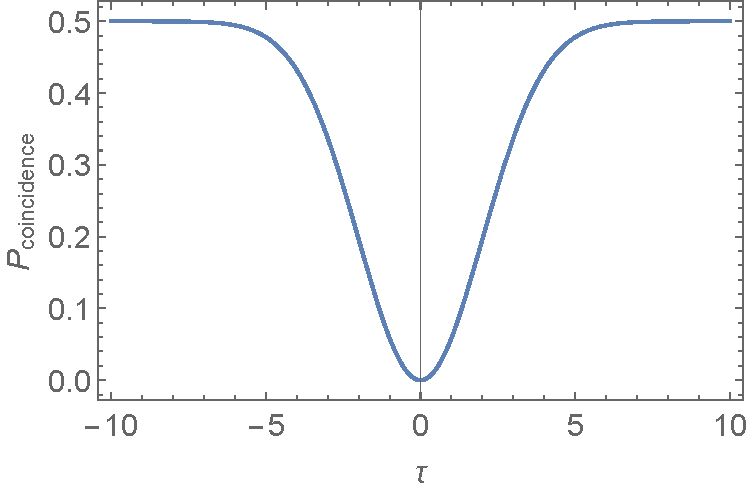
\includegraphics[clip=true, width=0.475\textwidth]{HOM_dip}
\captionspacefig \caption{Hong-Ou-Mandel dip for two photons with normal Gaussian temporal distribution functions, and temporal offset $\tau$ between them. $\tau$ effectively characterises the degree of photon distinguishability, where \mbox{$\tau=0$} represents complete indistinguishability (quantum statistics), and \mbox{$\tau\to\pm\infty$} represents complete distinguishability (classical statistics). Thus, performing this experiment and measuring $P_\mathrm{coincidence}$ can be used to characterise the degree of photon distinguishability.} \label{fig:HOM_dip}\index{Hong-Ou-Mandel (HOM) interference}
\end{figure}

In the above representation of mode-mismatch as a temporal or spatial translation, the process is entirely coherent, and could in principle be reversed if the translation were known (which might easily be established using tomographic characterisation techniques). Of course, such translations could occur incoherently also. In particular, `time-jitter' is where this process occurs incoherently, and the photons are subject to probabilistic temporal displacements. In this instance, a pure single-photon state would evolve into a mixture of states subject to different displacements. Since the mode-mismatch is now probabilisitic, it is not reversible. The state of a single photon subject to time-jitter would be of the form,
\begin{align}\index{Time-jitter}
\hat\rho_\mathrm{jitter} = \int_{-\infty}^\infty p_\mathrm{jitter}(\Delta_t) \ket{\psi-\Delta_t}\bra{\psi-\Delta_t}d\Delta_t,
\end{align}
where $p_\mathrm{jitter}(\Delta_t)$ characterises the classical probability distribution of the temporal displacement. Time-jitter is particularly natural in heralded spontaneous parametric down-conversion (SPDC) sources (Sec.~\ref{sec:single_phot_src}), where imprecision in the measurement time of the heralding mode projects that temporal uncertainty onto the heralded state. For this reason, much time is being invested into engineering SPDC sources with separable output photons, such that pathological behaviour of the detection of the heralding photon does not project the heralded photon onto a mixed state. Time-jitter is a major consideration in all present-day single-photon source technologies.

When considering mode-mismatch, there are two general regimes for how it manifests itself in an optical system. The first is when the interference taking place is between distinct, independent photons, i.e HOM interference (or its equivalent generalisations to higher-photon-number systems). The second is when multiple paths followed by a given photon interfere it with itself, i.e Mach-Zehnder (MZ)\index{Mach-Zehnder (MZ) interference} interference. The former only requires mode-matching on the scale of the photons' wave-packets, whereas the latter requires interferometric stability on the order of the photons' wavelength, a far more demanding requirement. This is discussed in greater detail in Sec.~\ref{sec:opt_stab}.

Mode-mismatch has been studied extensively in the context of linear optics quantum computing (LOQC), introduced in Sec.~\ref{sec:KLM_univ}. In particular, it was shown that in the cluster state formalism (Sec.~\ref{sec:CSQC}), mode-mismatch in a fusion gate is equivalent to a dephasing error model, where the dephasing rate is related to the degree of photon distinguishability (i.e visibility) \cite{bib:RohdeRalph06}. More generally, the operation of entangling gates \cite{bib:RohdeFreqTemp05, bib:RohdeGateChar05, bib:RohdeOptPhot05, bib:RohdeTimeRes11} and \textsc{BosonSampling} \cite{bib:RohdeArbSpec15, bib:RohdeArbLow12} have been considered, and explicit error models derived.

%
% Dispersion
%

\subsection{Dispersion} \label{sec:dispersion}\index{Dispersion}

Dispersion is the phenomenon of frequency-dependent velocity of light in a given medium. These effects can be very diverse, but can always be expressed in the mode-operator representation using an appropriate transformation in the temporal or spectral wavefunction,
\begin{align}
f_\mathrm{disp}: \,\tilde\psi(\omega)\to\tilde\psi(\omega)'.
\end{align}

%
% Spectral Filtering
%

\subsection{Spectral filtering} \label{sec:spectral_filt} \index{Spectral filtering}

In Sec.~\ref{sec:eff_err} we discussed the loss channel, whereby with some fixed probability photons are lost to the environment. In reality, this process is often not uniform, but frequency-dependent, resulting in spectral filtering effects. For example, optical fibres are typically designed to operate with a particular optical frequency in mind, and will attenuate frequencies outside a given range, implementing, for example, low-pass, high-pass or band-pass spectral filtering.

Because spectral filtering can be regarded as frequency-dependent loss, it can be modelled in the same way as per the loss channel, but using a frequency-dependent beamsplitter with transmissivity $\eta_f(\omega)$, which models the frequency response of the channel. The model is shown in Fig.~\ref{fig:spectral_filter_model}.

\begin{figure}[!htbp]
	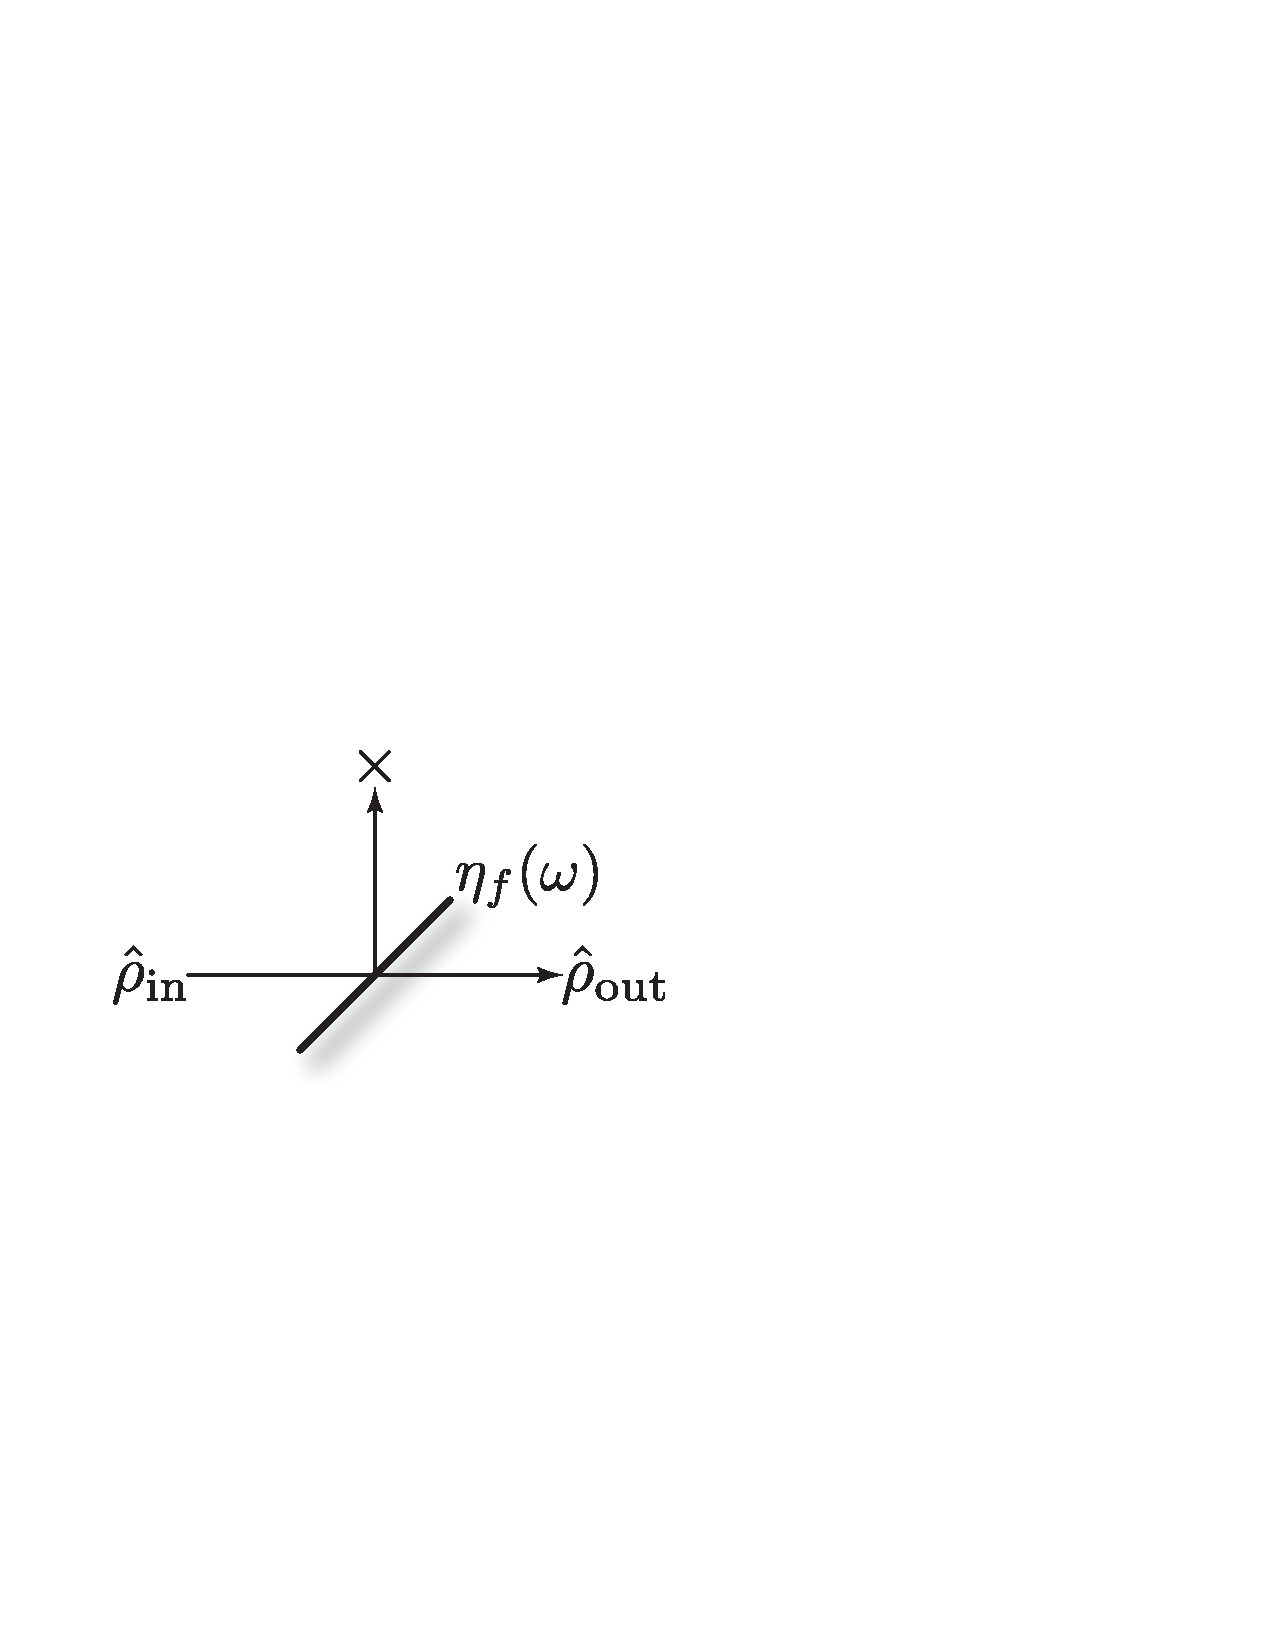
\includegraphics[clip=true, width=0.25\textwidth]{spectral_filter_model}
	\captionspacefig \caption{Model for the spectral filtering channel. The input state, $\hat\rho_\mathrm{in}$, passes through a beamsplitter of frequency-dependent transmissivity $\eta_f(\omega)$, and the reflected mode discarded, yielding the lossy output state \mbox{$\hat\rho_\mathrm{out} = \mathcal{E}^\mathrm{filter}_{\eta_f}(\hat\rho_\mathrm{in})$}.} \label{fig:spectral_filter_model} \index{Spectral filtering}
\end{figure}

This channel has the effect of modulating the spectral distribution function of a photonic mode operator $\hat{A}_\psi^\dag$ to $\hat{A}_{\psi'}^\dag$, where,
\begin{align}
\psi'(\omega) = \sqrt{\eta_f(\omega)}\psi(\omega).	
\end{align}
Note that unless \mbox{$\eta_f(\omega)=1\,\forall\,\,\psi(\omega)\neq 0$}, the new distribution function $\psi'(\omega)$ will not be normalised, where the normalisation reflects the loss probability,
\begin{align}
p_\mathrm{loss} = 1 - \int_{-\infty}^\infty \eta_f(\omega)|\psi(\omega)|^2\,d\omega.
\end{align}

%
% Phase-Space
%

\subsection{Phase-space} \index{Phase!Space!Errors}

In Sec.~\ref{sec:non_lin_opt} we introduce the displacement and squeezing operations, two non-linear operations which are important ingredients in CV quantum information processing schemes. Of course, such processes are subject to errors.

In the case of the displacement operation, which is implemented by mixing a state with a coherent state on a beamsplitter, errors in the amplitude of the coherent state or in the beamsplitter reflectivity will introduce an offset in the displacement amplitude. Thus, instead of implementing $\hat{D}(\alpha)$, we might over- or under-displace the state, implementing,
\begin{align}
	\hat{D}(\Delta)\hat{D}(\alpha)\propto \hat{D}(\alpha+\Delta),
\end{align}
for some error $\Delta$.

In the case of the squeezing operation, we might similarly have uncertainty in the squeezing parameter, thus implementing $\hat{S}(\xi+\Delta)$ instead of $\hat{S}(\xi)$.